\documentclass{beamer}

\usetheme{Berlin}

\usepackage{fontspec}
\usepackage{polyglossia}
\setmainlanguage{czech}

\usepackage{graphicx}
\usepackage{epstopdf}

\setlength{\unitlength}{0.5cm}

\title{Simulace SMP}
\author{Zdeněk Janeček \& Tomáš Cigler \& David Fiedler} 
\date{18.\,prosince 2015}

\begin{document}

\begin{frame} 
\titlepage
\end{frame}

\begin{frame} 
\frametitle{Zadání a úvod}
Vytvořte simulátor čtyřjádrového SMP a k němu:

\begin{itemize}
\item plánovač
\item synchronizaci procesů (semafory)
\item úlohu producent-konzument (poběží v osmi instancích)
\item rozhraní pro řízení procesoru a spuštěných úloh
\end{itemize}

\end{frame}


\begin{frame} 
\frametitle{Návrh implementace}

\begin{itemize}
\item start podobný jako start systému
\item inicializace systému obsluh přerušení
\item běh procesoru - jedna INIT úloha
\item inicializace úloh producent-konzument do plánovače
\item plánování na základě přerušení a časového kvanta (Round Robin)
\end{itemize}


\end{frame}

\begin{frame} 
\frametitle{Rozhraní}

Konzole jako ovládací a monitorovací rozhraní:

\begin{itemize}
\item exit: vypne program
\item start: spustí úlohu
\item help: ukáže nápovědu
\item show: ukáže informace o~běžících procesech,čekajících procesech a obsazenosti CPU
\item state: zobrazí aktuální chybu výpočtu v~úlohách. Tato funkce je volána pravidelně.
\item pause-core: pozastaví jádro procesoru
\item resume-core: znovu spustí jádro procesoru
\end{itemize}

\end{frame}

\begin{frame} 
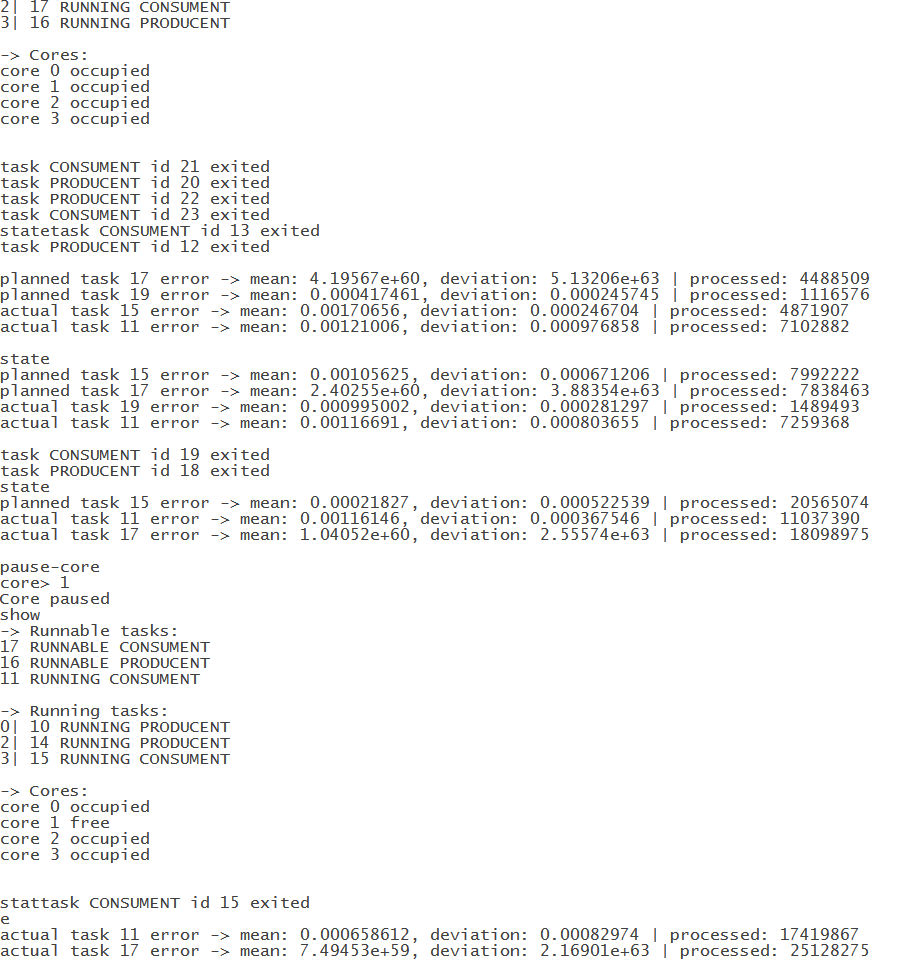
\includegraphics[height=\textheight]{obrazky/screen.png}

\end{frame}

\begin{frame}
\frametitle{SMP bootstrap}

\begin{itemize}
\item hardwarové hodiny plánovače
\begin{itemize}
  \item SMP init - vytvoří interrupt thread, pracovní vlákno
  \item SMP terminate
  \item spustí pravidelné přerušení plánovačem
\end{itemize}
\item plánovač

\begin{itemize}
  \item vytvoří si vlastní zásobník
  \item default\_context
\end{itemize}
\end{itemize}
\end{frame}

\begin{frame}
\frametitle{Přerušení}

\begin{columns}
  \begin{column}{0.5\textwidth}
\begin{block}{Součásti}
\begin{itemize}
  \item Event handler
  \item maska
  \item message DWORD
  \item obslužná rutina
\end{itemize}
\end{block}
  \end{column}

  \begin{column}{0.5\textwidth}
\begin{block}{Druhy}
\begin{itemize}
  \item plánovač
  \item přeplánování
  \item zastavení jádra --- Pause
  \item obnovení jádra --- Resume
  \item ukončení --- Terminate
\end{itemize}
\end{block}
  \end{column}
\end{columns}

\end{frame}

\begin{frame}[fragile]
\frametitle{Přepínání kontextu}

Přepnutí probíhá odlišně z interrupt thread a při \emph{in place} přerušení.
\begin{itemize}
\item cílové ESP (buď rovnou změnou kontextu a nebo jako návratová hodnota plánovače)
\item a skok na EIP obsluhy
\item kontext je obnoven pomocí pop ze zásobníku
\end{itemize}

\begin{verbatim}
DWORD target_esp = (DWORD)next_task->context.Esp;
__asm {
  mov esp, target_esp
  jmp do_reschedule
do_reschedule:
  popad
  popfd
  ret }
\end{verbatim}
\end{frame}

\begin{frame}
\frametitle{Plánovač}

Stará se o:
\begin{itemize}
  \item vytvoření TCB pro nové úlohy
  \item smazání starých úloh
  \item ošetřit pozastavení (úloha jde do fronty) a obnovení jádra
  \item pro každý procesor
  \begin{itemize}
    \item sníží časové kvantum běžící úlohy
    \item \texttt{task\_queue}
    \item idle task na prvním jádře (spuštění v případě prázdné fronty)
    \item přepnutí úloh na všech procesorech
  \end{itemize}

\end{itemize}
Pro uchování pointerů jsme využili \texttt{std::unique\_ptr}.
\end{frame}

\begin{frame} %[fragile]
\frametitle{Úlohy}
\begin{itemize}
\item Dodělám zítra ráno
\end{itemize}
\end{frame}

\begin{frame} 
\frametitle{Výsledky a závěr}

\end{frame}

\end{document}
